\documentclass[twocolumn=on,DIV=calc]{scrartcl}
\usepackage[portuguese]{babel}
\usepackage[colorlinks,allcolors=blue]{hyperref}
\usepackage[utf8]{inputenc}
\usepackage{microtype}
\usepackage[labelsep=period]{caption}
\usepackage{amsmath}
\usepackage{graphicx}
\newcommand{\dpar}[1]{\left(#1\right)}
\newcommand{\un}[1]{\mathrm{#1}}

\DeclareMathOperator{\sen}{sen}
\DeclareMathOperator{\pr}{pr}

\title{Física Geral I: Lista de exercícios 5}

\author{Data de entrega: 27 de junho de 2018}

\date{}

\begin{document}
\maketitle

\paragraph{Instruções}

\begin{itemize}
\item Fazer a questão correspondente ao último algarismo do seu RA. Se
  esse for $0$, faça a questão 10.
\item Além da questão anterior, faça uma outra questão de sua escolha.
\end{itemize}

\paragraph{Questões}


\begin{enumerate}
\item A figura~\ref{fig:1} mostra um arame em forma de $V$ e um anel
  de massa $m$ que pode deslizar por uma das partes do arame sem
  atrito. Determine o valor da velocidade angular constante $\omega$
  para que o anel permaneça girando a uma altura $h=1\,\un{m}$.
  \begin{figure}[ht]
    \centering
    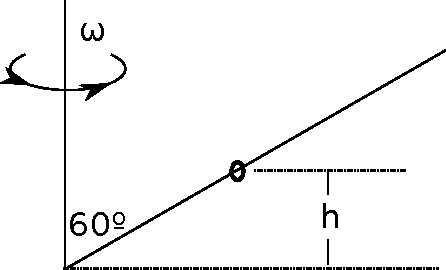
\includegraphics[width=0.4\textwidth,keepaspectratio]{lista5-questao1.pdf}
    \caption{}
    \label{fig:1}
  \end{figure}
\item A figura~\ref{fig:2} mostra uma esfera $A$ sobre uma mesa a qual
  está unida a uma outra esfera $B$ por uma corda que passa por um
  orifício da mesa. A esfera $A$ desliza sem atrito sobre a mesa
  realizando um movimento circular uniforme de raio
  $R=0.5\,\un{m}$. Se as massas das esferas são $m_A=0.2\,\un{kg}$ e
  $m_B=2\,\un{kg}$ e a esfera $B$ está a uma certa altura do chão,
  determine o módulo da velocidade da esfera $A$ para que a esfera $B$
  não caia.
  \begin{figure}[ht]
    \centering
    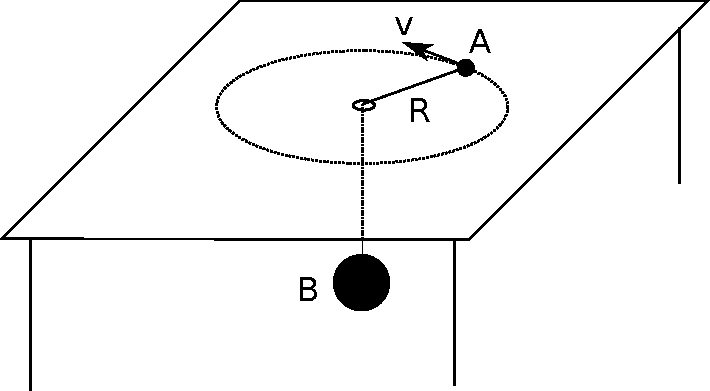
\includegraphics[width=0.4\textwidth,keepaspectratio]{lista5-questao2.pdf}
    \caption{}
    \label{fig:2}
  \end{figure}
\item Uma força de $20\,\un N$ é aplicada sobre um bloco de
  $5\,\un{kg}$, inicialmente em repouso, que pode deslizar por uma
  superfície reta que tem uma parte lisa e outra rugosa (ver
  figura~\ref{fig:3}). (i)~Se a distância entre os pontos $1$ e $2$
  (parte lisa) é de $4\,\un{m}$, determine a velocidade do bloco no
  ponto $2$. (ii)~Se depois do ponto $2$ não se aplica mais a força
  sobre o bloco, determine a distância que ele percorre na parte
  rugosa até se deter, sabendo que o coeficiente de atrito cinético
  nessa parte é $\mu_c=0.8$.
  \begin{figure}[ht]
    \centering
    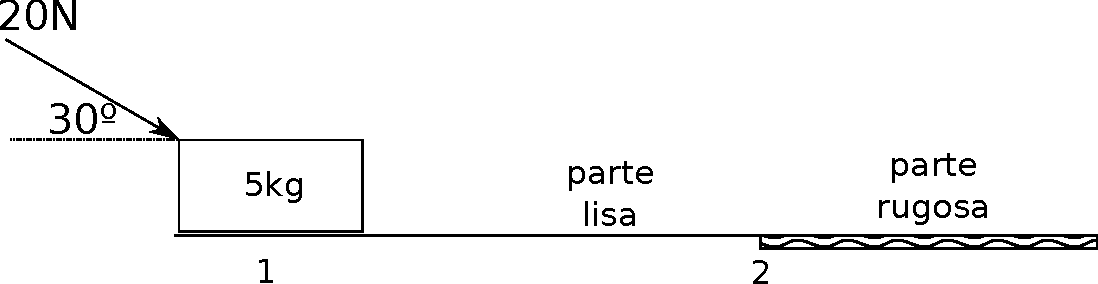
\includegraphics[width=0.4\textwidth,keepaspectratio]{lista5-questao3.pdf}
    \caption{}
    \label{fig:3}
  \end{figure}
\end{enumerate}
\end{document}